\documentclass[tikz,border=4pt]{standalone}
\usepackage{mathptmx}
\usetikzlibrary{positioning,arrows.meta,fit,backgrounds}
\begin{document}
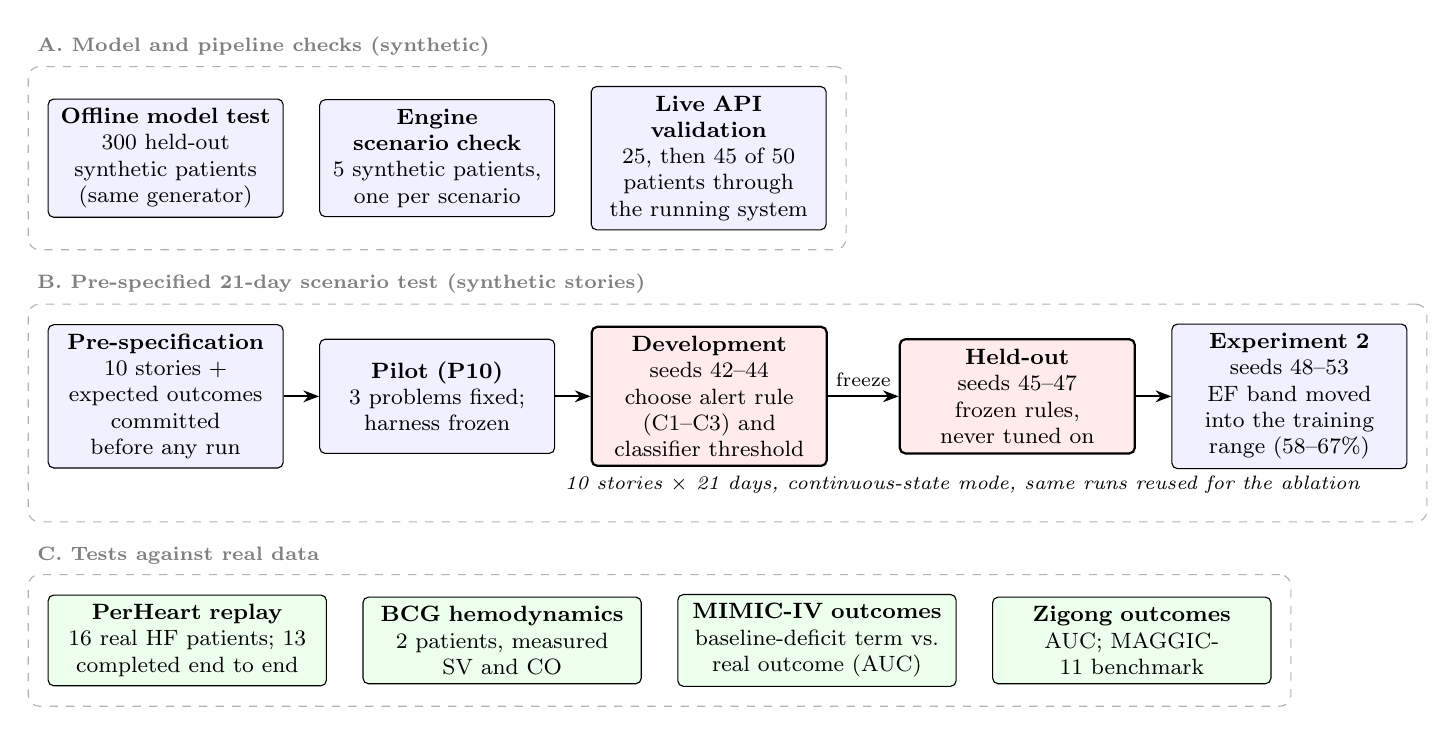
\begin{tikzpicture}[font=\footnotesize, node distance=0.45cm,
  st/.style={execute at begin node={\hyphenpenalty=10000\relax}, draw, rounded corners=2pt, fill=blue!6, align=center, text width=2.75cm, minimum height=1.45cm},
  key/.style={st, fill=red!8, thick},
  real/.style={execute at begin node={\hyphenpenalty=10000\relax}, draw, rounded corners=2pt, fill=green!7, align=center, text width=3.3cm, minimum height=1.1cm},
  flow/.style={-{Stealth[length=2mm]}, thick},
  lane/.style={draw=gray!60, dashed, rounded corners=4pt, inner sep=7pt}]
% lane 1: model and pipeline checks
\node[st] (off) {\textbf{Offline model test}\\300 held-out synthetic patients\\(same generator)};
\node[st, right=of off] (eng) {\textbf{Engine scenario check}\\5 synthetic patients,\\one per scenario};
\node[st, right=of eng] (api) {\textbf{Live API validation}\\25, then 45 of 50 patients through the running system};
% lane 2: pre-specified scenario test
\node[st, below=1.35cm of off] (pre) {\textbf{Pre-specification}\\10 stories + expected outcomes committed before any run};
\node[st, right=of pre] (pil) {\textbf{Pilot (P10)}\\3 problems fixed;\\harness frozen};
\node[key, right=of pil] (dev) {\textbf{Development}\\seeds 42--44\\choose alert rule (C1--C3) and classifier threshold};
\node[key, right=0.9cm of dev] (held) {\textbf{Held-out}\\seeds 45--47\\frozen rules, never tuned on};
\node[st, right=of held] (exp2) {\textbf{Experiment 2}\\seeds 48--53\\EF band moved into the training range (58--67\%)};
\draw[flow] (pre) -- (pil);
\draw[flow] (pil) -- (dev);
\draw[flow] (dev) -- node[above, font=\scriptsize] {freeze} (held);
\draw[flow] (held) -- (exp2);
\node[font=\scriptsize\itshape, below=0.15cm of pil.south east, anchor=north west] (note) {10 stories $\times$ 21 days, continuous-state mode, same runs reused for the ablation};
% lane 3: real data
\node[real, below=1.6cm of pre.south west, anchor=north west] (ph) {\textbf{PerHeart replay}\\16 real HF patients; 13 completed end to end};
\node[real, right=of ph] (bcg) {\textbf{BCG hemodynamics}\\2 patients, measured SV and CO};
\node[real, right=of bcg] (mimic) {\textbf{MIMIC-IV outcomes}\\baseline-deficit term vs.\ real outcome (AUC)};
\node[real, right=of mimic] (zg) {\textbf{Zigong outcomes}\\AUC; MAGGIC-11 benchmark};
% lane boxes
\begin{scope}[on background layer]
\node[lane, fit=(off)(eng)(api), label={[anchor=south west, font=\scriptsize\bfseries, gray]north west:A. Model and pipeline checks (synthetic)}] {};
\node[lane, fit=(pre)(pil)(dev)(held)(exp2)(note), label={[anchor=south west, font=\scriptsize\bfseries, gray]north west:B. Pre-specified 21-day scenario test (synthetic stories)}] {};
\node[lane, fit=(ph)(bcg)(mimic)(zg), label={[anchor=south west, font=\scriptsize\bfseries, gray]north west:C. Tests against real data}] {};
\end{scope}
\end{tikzpicture}
\end{document}
